%----------------------------------------------------------------------------------------
%    PACKAGES AND THEMES
%----------------------------------------------------------------------------------------

\documentclass[aspectratio=169,xcolor=dvipsnames]{beamer}
\usetheme{SimpleDarkBlue}

\usepackage{hyperref}
\usepackage[utf8]{inputenc}  
\usepackage{graphicx} % Allows including images
\usepackage{tikz}
\usepackage{booktabs} % Allows the use of \toprule, \midrule and \bottomrule in tables
\usepackage{amsmath}
\usepackage{bm}
\usepackage{subcaption}
\usepackage{braket}     
%----------------------------------------------------------------------------------------
%    TITLE PAGE
%----------------------------------------------------------------------------------------

\title{Implementación de canales cuánticos de un qubit usando Algoritmos Variacionales Cuánticos}
    \author{Felipe Ixcamparic \\
\textbf{Asesores:} Dr. Carlos Pineda y Dr. Giovanni Ramírez}

\institute
{
    Escuela de Ciencias Físicas y Matemáticas \\
    Universidad de San Carlos de Guatemala \\ 
    Instituto de Física \\
    Universidad Nacional Autónoma de México % Your institution for the title page
}
\date{\today} % Date, can be changed to a custom date
\titlegraphic{%
\begin{tikzpicture}[remember picture,overlay]
  \node[anchor=south west,xshift=0.5cm,yshift=0.5cm]
    at (current page.south west) {
\includegraphics[height=1.8cm]{imagenes/ECFM_logo.png}};
  \node[anchor=south east,xshift=-0.5cm,yshift=0.5cm]
    at (current page.south east) {
\includegraphics[height=1.5cm]{imagenes/IF_logo.png}};
\end{tikzpicture}
}

%----------------------------------------------------------------------------------------
%    PRESENTATION SLIDES
%----------------------------------------------------------------------------------------

\begin{document}

\begin{frame}
    % Print the title page as the first slide
    \titlepage
\end{frame}

\begin{frame}{Overview}
    % Throughout your presentation, if you choose to use \section{} and \subsection{} commands, these will automatically be printed on this slide as an overview of your presentation
    \tableofcontents
\end{frame}

%------------------------------------------------
\section{Introducción}
%------------------------------------------------

\begin{frame}{Introducción}
    \begin{itemize}
        \item Lorem ipsum dolor sit amet, consectetur adipiscing elit
        \item Aliquam blandit faucibus nisi, sit amet dapibus enim tempus eu
        \item Nulla commodo, erat quis gravida posuere, elit lacus lobortis est, quis porttitor odio mauris at libero
        \item Nam cursus est eget velit posuere pellentesque
        \item Vestibulum faucibus velit a augue condimentum quis convallis nulla gravida
    \end{itemize}
    
\end{frame}

%------------------------------------------------

\begin{frame}{Blocks of Highlighted Text}
    In this slide, some important text will be \alert{highlighted} because it's important. Please, don't abuse it.

    \begin{block}{Block}
        Sample text
    \end{block}

    \begin{alertblock}{Alertblock}
        Sample text in red box
    \end{alertblock}

    \begin{examples}
        Sample text in green box. The title of the block is ``Examples".
    \end{examples}
\end{frame}

%------------------------------------------------

\begin{frame}{Multiple Columns}
    \begin{columns}[c] % The "c" option specifies centered vertical alignment while the "t" option is used for top vertical alignment

        \column{.45\textwidth} % Left column and width
        \textbf{Heading}
        \begin{enumerate}
            \item Statement
            \item Explanation
            \item Example
        \end{enumerate}

        \column{.45\textwidth} % Right column and width
        Lorem ipsum dolor sit amet, consectetur adipiscing elit. Integer lectus nisl, ultricies in feugiat rutrum, porttitor sit amet augue. Aliquam ut tortor mauris. Sed volutpat ante purus, quis accumsan dolor.

    \end{columns}
\end{frame}

%------------------------------------------------
\section{Conceptos Fundamentales (Pendiente) }
%------------------------------------------------

\begin{frame}{Table}
    \begin{table}
        \begin{tabular}{l l l}
            \toprule
            \textbf{Treatments} & \textbf{Response 1} & \textbf{Response 2} \\
            \midrule
            Treatment 1         & 0.0003262           & 0.562               \\
            Treatment 2         & 0.0015681           & 0.910               \\
            Treatment 3         & 0.0009271           & 0.296               \\
            \bottomrule
        \end{tabular}
        \caption{Table caption}
    \end{table}
\end{frame}

%------------------------------------------------

\begin{frame}{Theorem}
    \begin{theorem}[Mass--energy equivalence]
        $E = mc^2$
    \end{theorem}
\end{frame}

%------------------------------------------------

\begin{frame}{Figure}
    Uncomment the code on this slide to include your own image from the same directory as the template .TeX file.
    %\begin{figure}
    %\includegraphics[width=0.8\linewidth]{test}
    %\end{figure}
\end{frame}

%------------------------------------------------

\begin{frame}[fragile] % Need to use the fragile option when verbatim is used in the slide
    \frametitle{Citation}
    An example of the \verb|\cite| command to cite within the presentation:\\~

    This statement requires citation \cite{p1}.
\end{frame}



\section{Algoritmos Variacionales Cuánticos}
%------------------------------------------------

\begin{frame}{Algoritmos Variacionales Cuánticos}
\begin{itemize}
    \item Combinan computación cuántica y optimización clásica para resolver tareas específicas.
    
    \item Se basan en un circuito cuántico parametrizado $U(\bm{\theta})$ aplicado sobre un estado inicial $\ket{\psi_0}$:
    \begin{equation*}
    \ket{\psi(\bm{\theta})} = U(\bm{\theta}) \ket{\psi_0},   
    \end{equation*}    
    donde $\bm{\theta}$ es optimizado para minimizar una función de costo $C(\bm{\theta})$.
    
    \item Buscan:
    \begin{equation*}
        \bm{\theta}^* = \underset{\bm{\theta}}{\text{arg min}}\, C(\bm{\theta}).        
    \end{equation*}
\end{itemize}
\end{frame}

%-------------------------------------------------
\begin{frame}{Algoritmos Variacionales Cuánticos}
\framesubtitle{Hardware Efficient Ansatz (HEA)}
\begin{columns}[c]
\column{.60\textwidth} 
    \begin{itemize}
        \item El \textit{ansatz} define la estructura de $U(\bm{\theta})$ , así como el tipo de compuertas cuánticas.
       
        \item El HEA usa compuertas nativas del dispositivo cuántico, además son agnósticos al problema a resolver.
       
        \item Escogimos el HEA:
        \begin{equation*}
        \label{ec:ansatz}
             U(\bm{\theta}) =\prod_{i=1}^{M} \prod_{j=1}^N U_{ent} (\theta_i)R_z(\theta_{ij})R_x(\theta_{ij2})R_z(\theta_{ij3}).
         \end{equation*}
    \end{itemize}
    
\column{0.5\textwidth}
    \begin{center}
        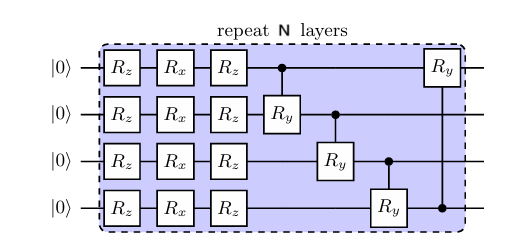
\includegraphics[width=1\linewidth]{imagenes/hu liu.png}
    \end{center}
\end{columns}
\end{frame}


\begin{frame}{Algoritmos Variacionales Cuánticos}
\framesubtitle{Implementación de Canales Cuánticos}
        \begin{figure}
            \centering
            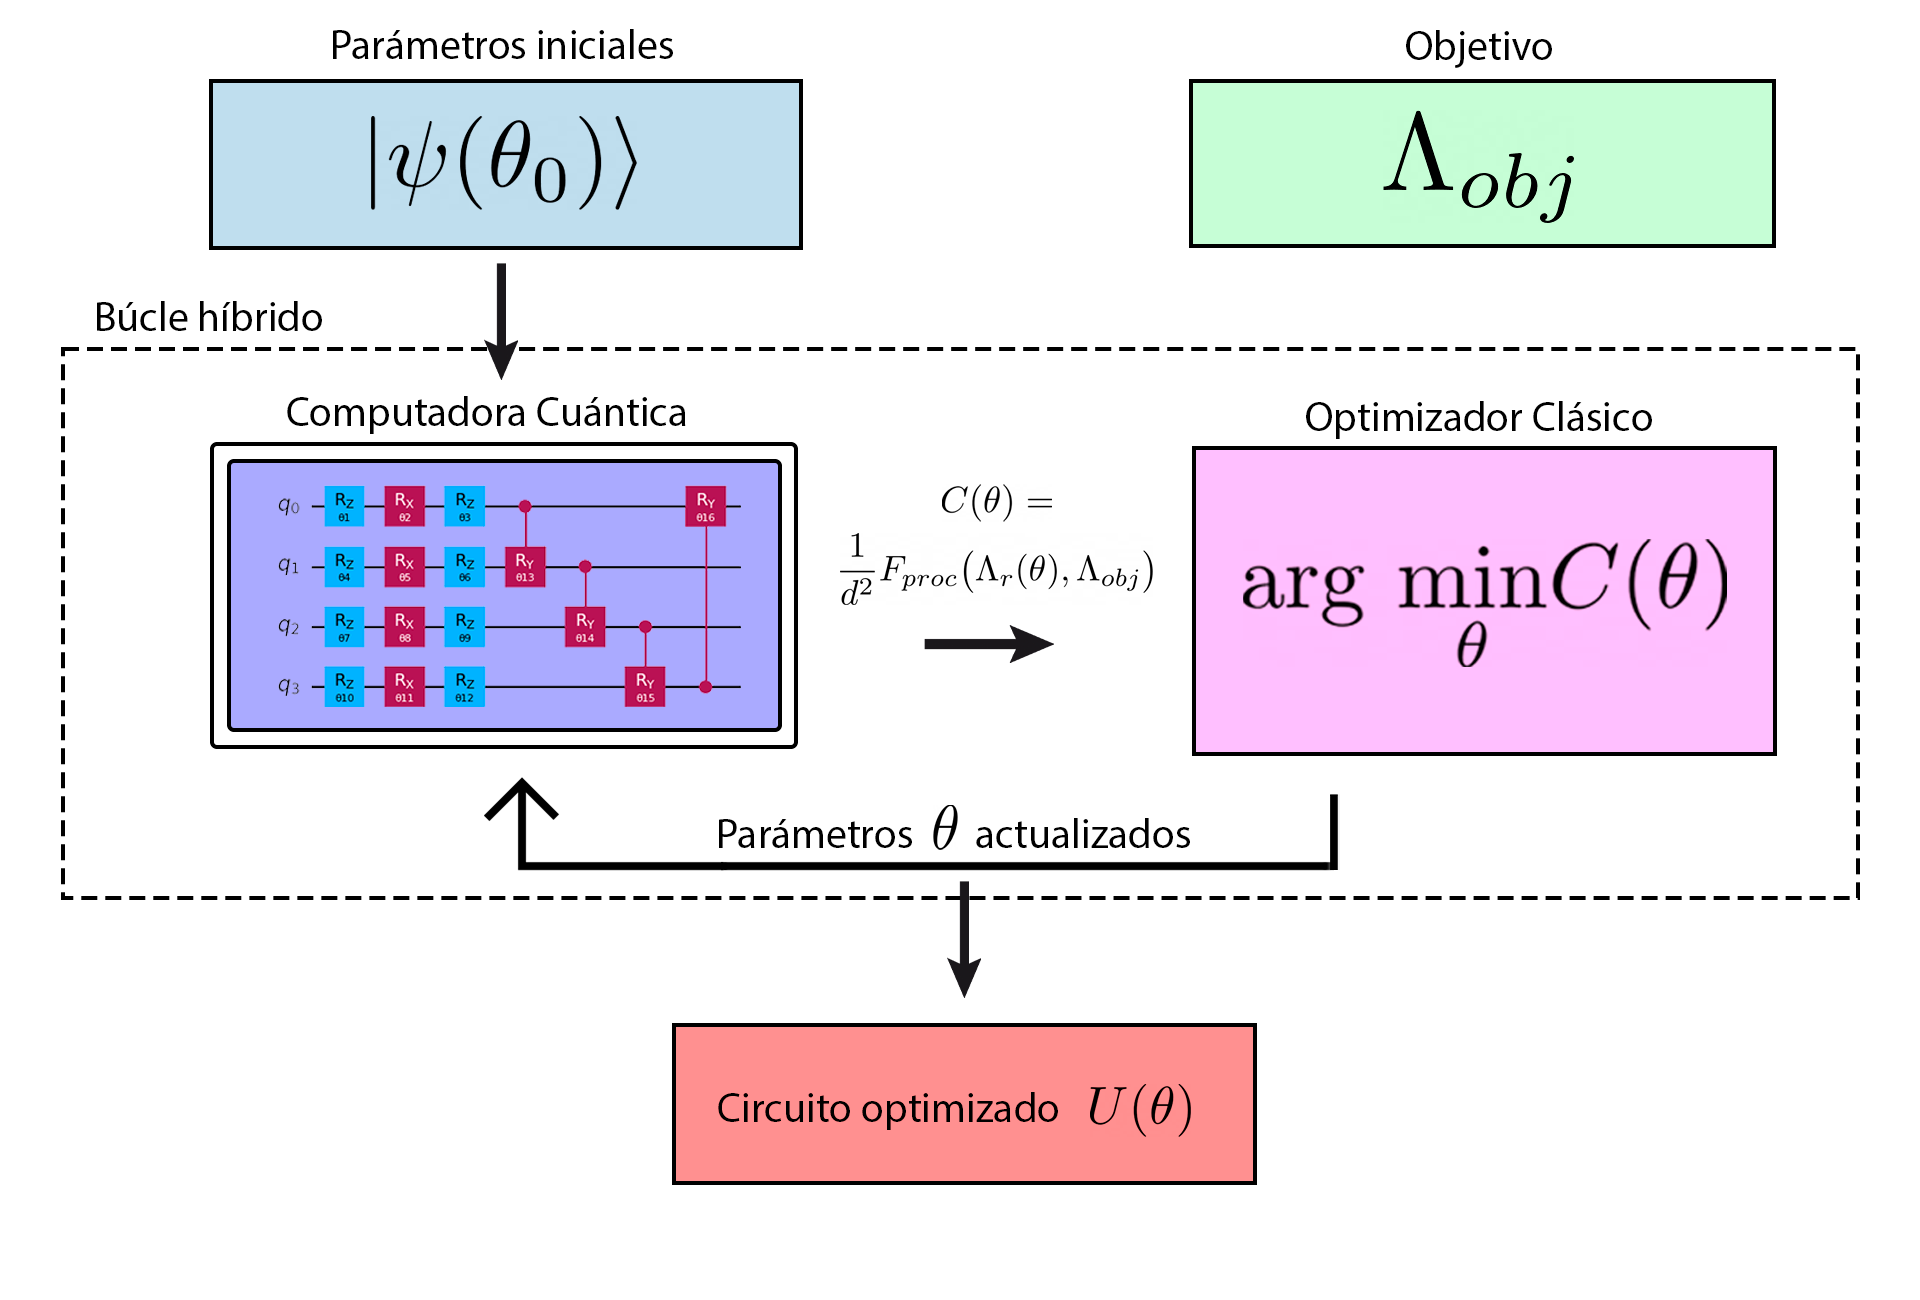
\includegraphics[width=0.75\linewidth]{imagenes/esquema_dp_v1.png}
            \label{fig:placeholder}
        \end{figure}
\end{frame}

\section{Resultados para el Canal Despolarizante de un qubit}
%------------------------------------------------

\begin{frame}{Resultados}
\framesubtitle{Canal Despolarizante}
    \begin{columns}[c] 

        \column{.60\textwidth} % Left column and width
    \begin{itemize}
        \item Modelo de ruido cuántico con probabilidad $p$ de convertir $\rho$ en $\frac{{I}}{2}$ mediante 
        \begin{equation*}
            \mathcal{E(\rho)}= \text{Tr}(\rho) p \frac{I}{2} + (1-p) \rho.
            \end{equation*}
  \item {} 
  \begin{equation*}\label{eq:choi_depolarizing}
    \Lambda_{\mathcal E}=\Lambda_{\text{obj}}=
    \begin{pmatrix}
      1-\frac{p}{2} & 0 & 0 & 1-p \\
      0 & \frac{p}{2} & 0 & 0 \\
      0 & 0 & \frac{p}{2} & 0 \\
      1-p & 0 & 0 & 1-\frac{p}{2}
    \end{pmatrix}.
  \end{equation*}
    \end{itemize}

        \column{.45\textwidth} % Right column and width
        \begin{figure}
            \centering
            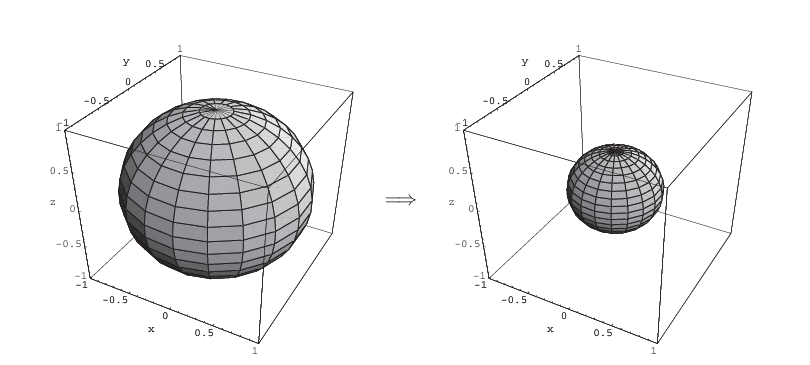
\includegraphics[width=1\linewidth]{imagenes/efecto_depolarizing.png}
            \label{fig:placeholder}
        \end{figure}
    \end{columns}
\end{frame}

% \begin{frame}{Table}
%     \begin{table}
%         \begin{tabular}{l l l}
%             \toprule
%             \textbf{Treatments} & \textbf{Response 1} & \textbf{Response 2} \\
%             \midrule
%             Treatment 1         & 0.0003262           & 0.562               \\
%             Treatment 2         & 0.0015681           & 0.910               \\
%             Treatment 3         & 0.0009271           & 0.296               \\
%             \bottomrule
%         \end{tabular}
%         \caption{Table caption}
%     \end{table}
% \end{frame}
% %------------------------------------------------

\begin{frame}{Resultados}
\framesubtitle{Restricciones y ejecuciones}
  \begin{itemize}
    \item Fijamos hiperparámetros: HEA de 1 capa y 2 qubits.
    \begin{center}
            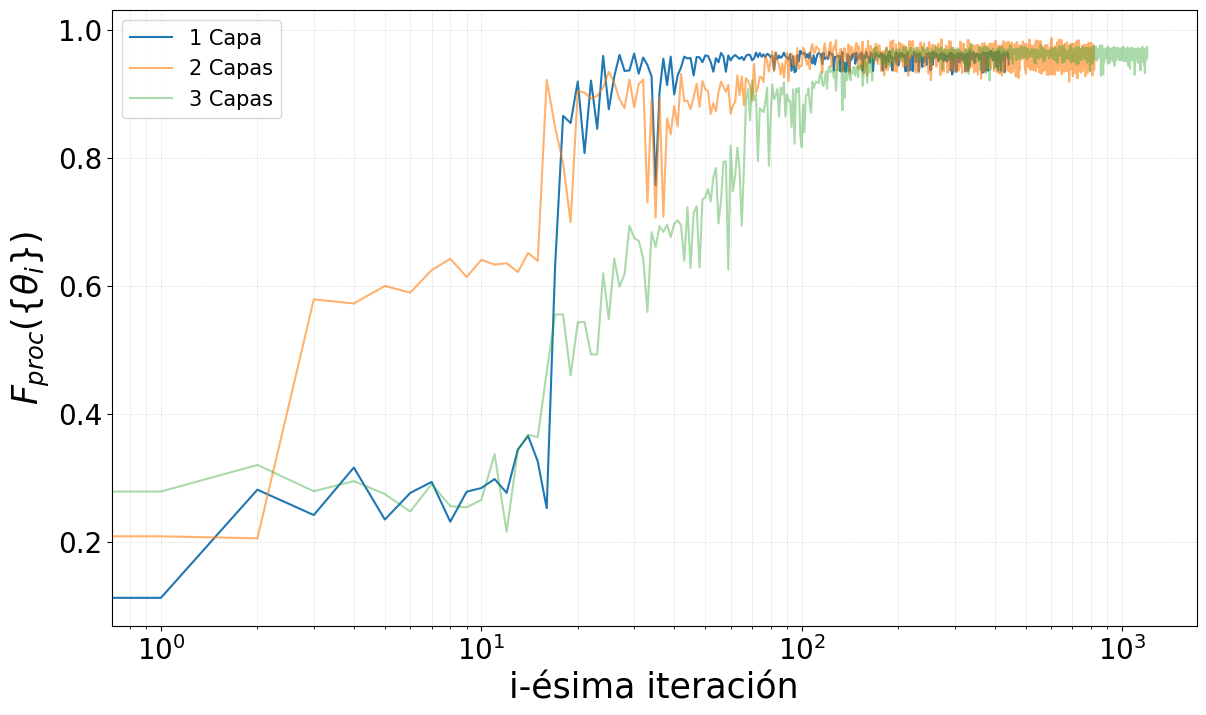
\includegraphics[width=0.60\textwidth]{imagenes/comparacion_capas.png}
          \end{center}
    % \item Tiempo máximo de ejecución (gratuito) mensual: 10 minutos.
    % \item Ejecución promedio por tomografía de proceso: 16 segundos.
    % \item Validación con tomografía 4 veces en simulador cuántico y 1 vez en computadora cuántica.
    % \item Ejecutamos para 38 valores distintos de $p$.
  \end{itemize}
\end{frame}


%=======================================================
\begin{frame}{Resultados}
\framesubtitle{Fidelidades}
    \begin{columns}[c] % The "c" option specifies centered vertical alignment while the "t" option is used for top vertical alignment

        \column{.60\textwidth} % Left column and width
\begin{figure}[h]
    \centering
    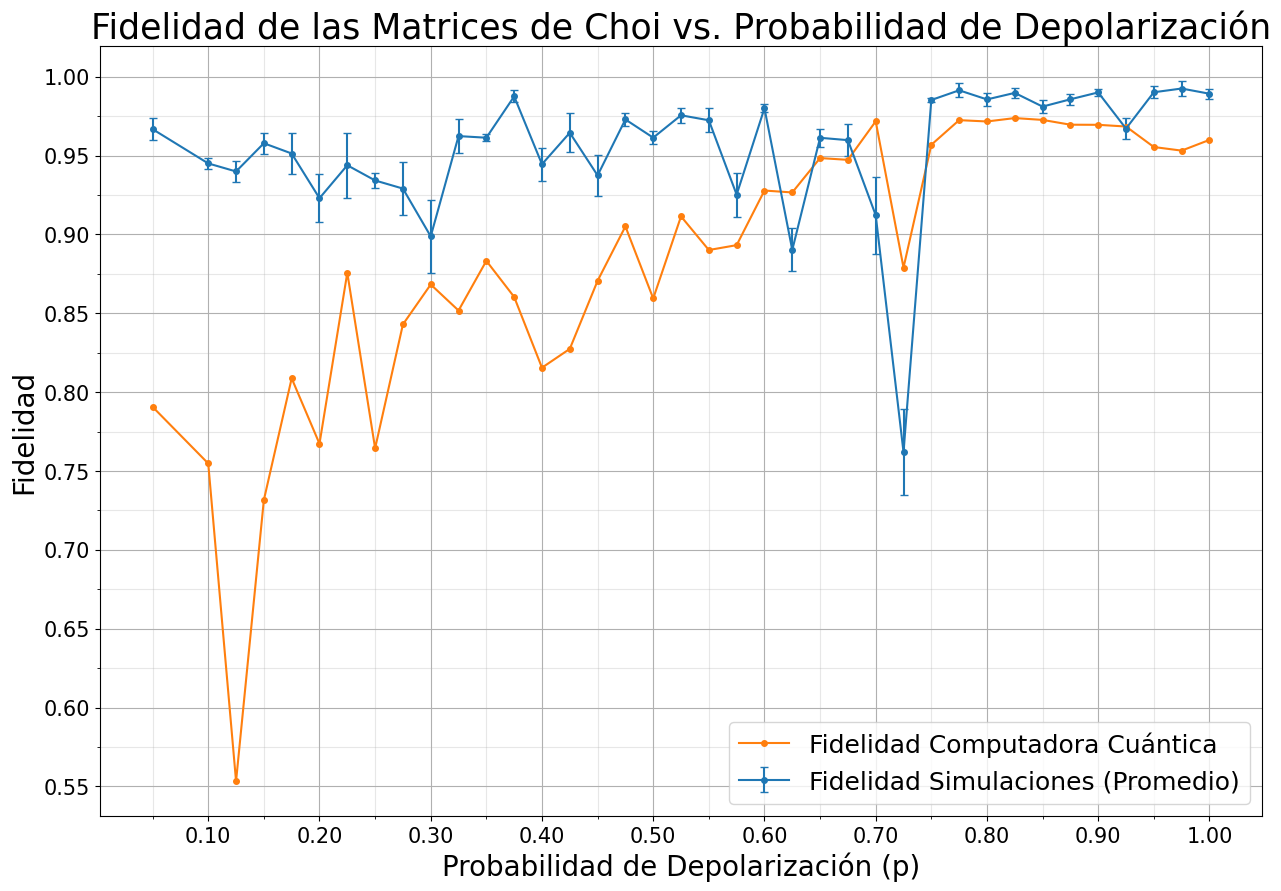
\includegraphics[scale=0.25]{imagenes/comparacion fidelidad.png}
    \label{fig:Bloch}
\end{figure}
        \column{.45\textwidth} % Right column and width
\begin{table}[htbp]
\centering 
\resizebox{\textwidth}{!}{
\begin{tabular}{|l|c|c|}
\hline
\textbf{Métrica} & \textbf{Aer Simulator} & \textbf{ibm-kyoto} \\ \hline
Mediana           & 0.9618 & 0.8916 \\ \hline
Mínimo            & 0.7620 & 0.5533 \\ \hline
Máximo            & 0.9925 & 0.9738 \\ \hline
p(max)            & 0.975  & 0.825  \\ \hline
p(min)            & 0.725  & 0.125  \\ \hline
Desv. Estándar    & 0.0418 & 0.0899 \\ \hline
\end{tabular}
}
\label{tab:comparacion_fidelidades}
\end{table}
    \end{columns}
\end{frame}
%=================================================================

\begin{frame}{Resultados}
\framesubtitle{Completa Positividad}
\begin{figure}[h!] 
    \centering 
    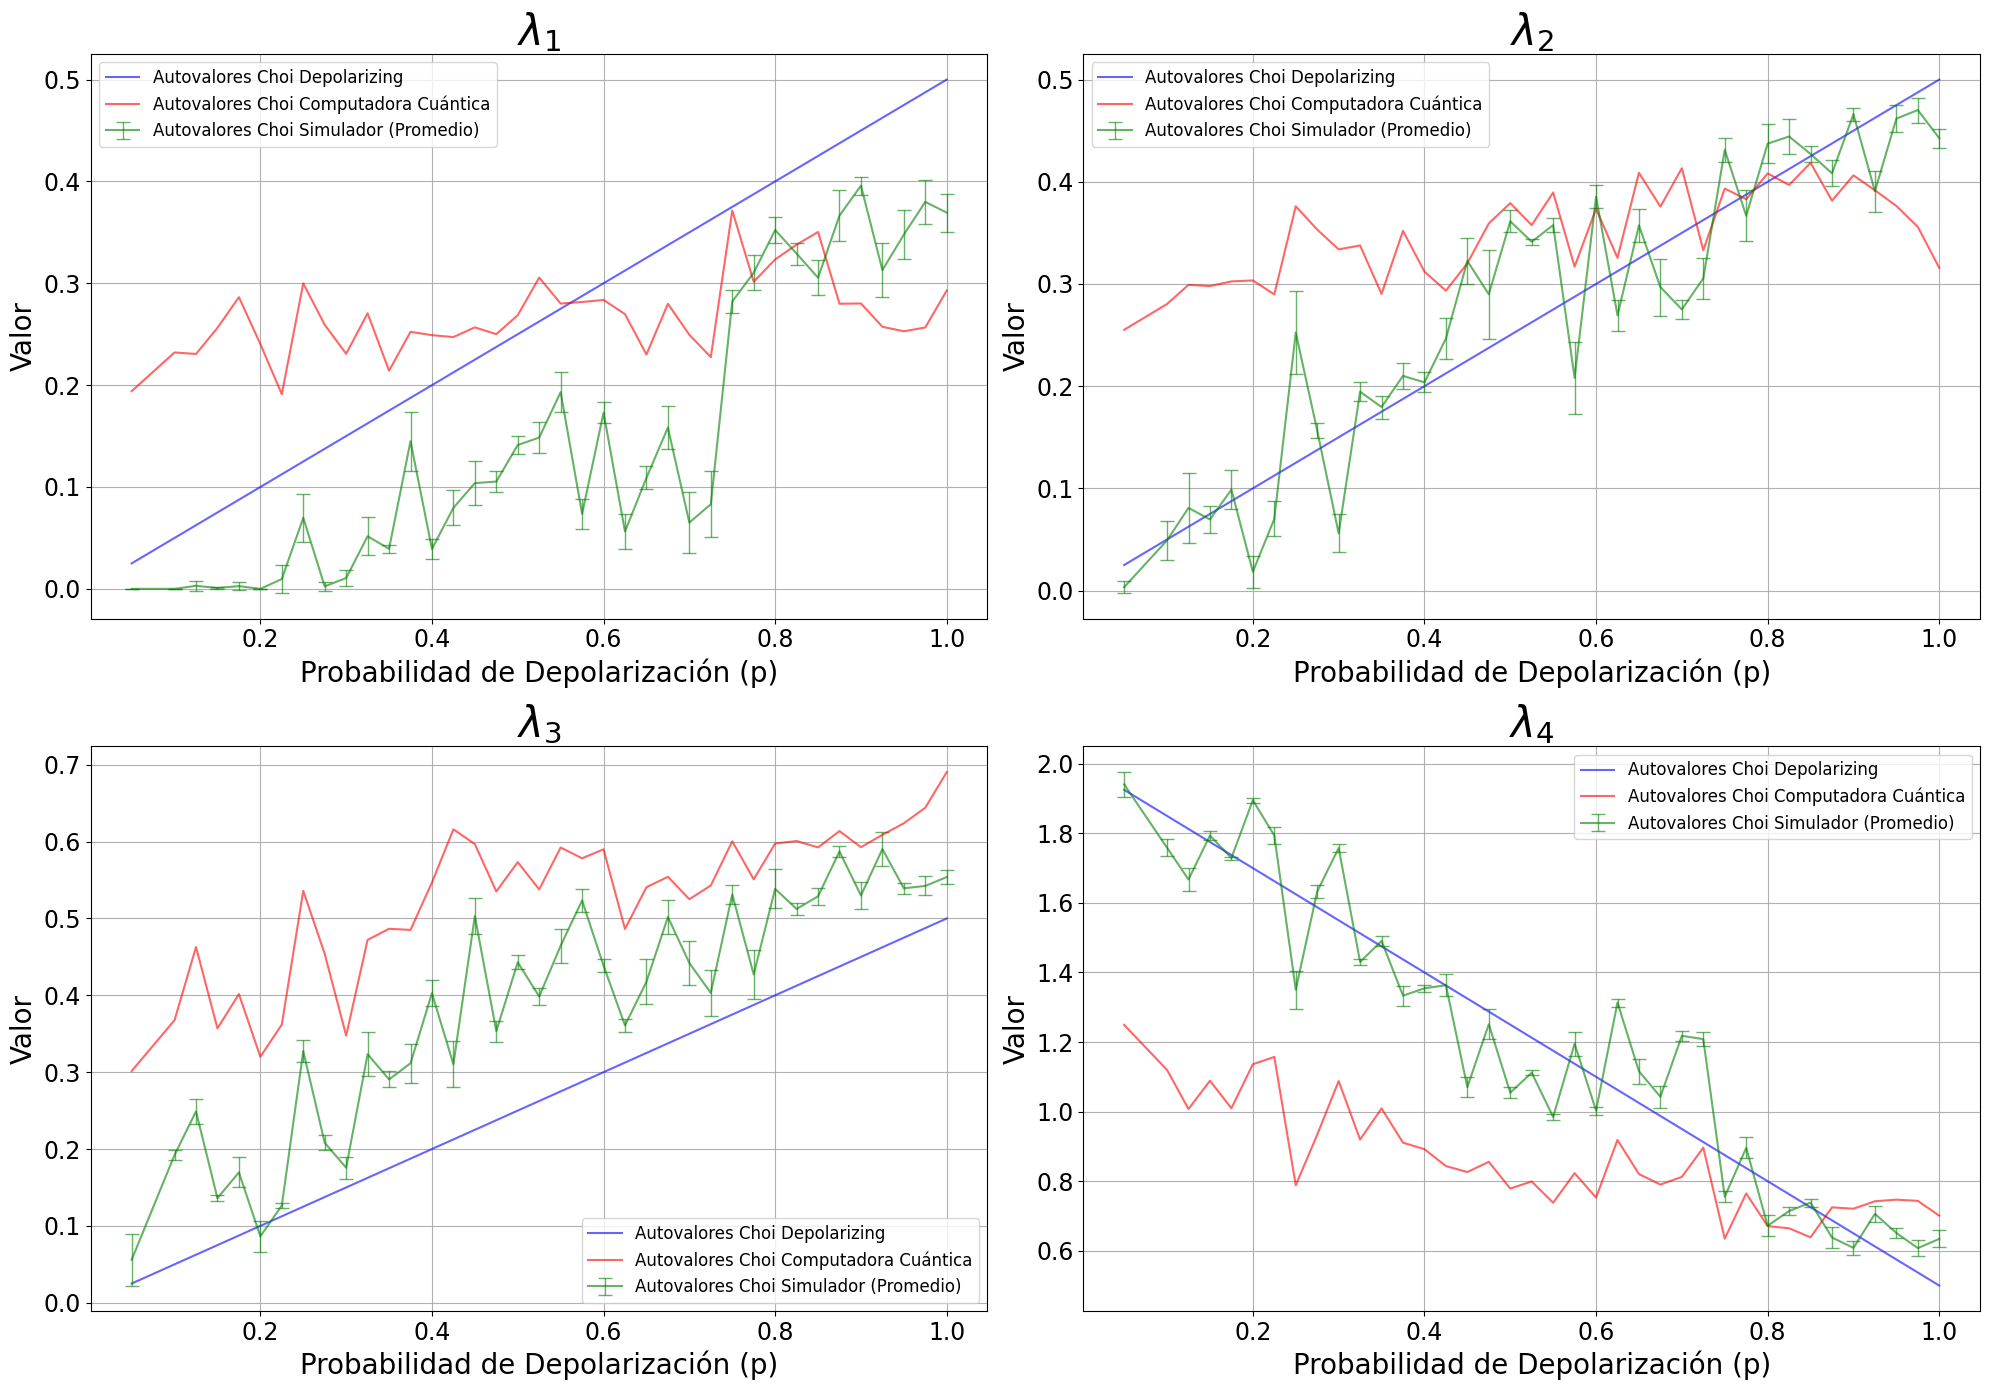
\includegraphics[width=0.7 \linewidth]{imagenes/eigenvalores_comparacion.png}
    \label{fig:comparacion_autovalores}
\end{figure}
\end{frame}


\begin{frame}{Resultados}
\framesubtitle{Preservación de la Traza}
\begin{figure}
  \centering

  % ===== Fila 1 =====
  \begin{subfigure}[t]{0.50\textwidth}
    \centering
    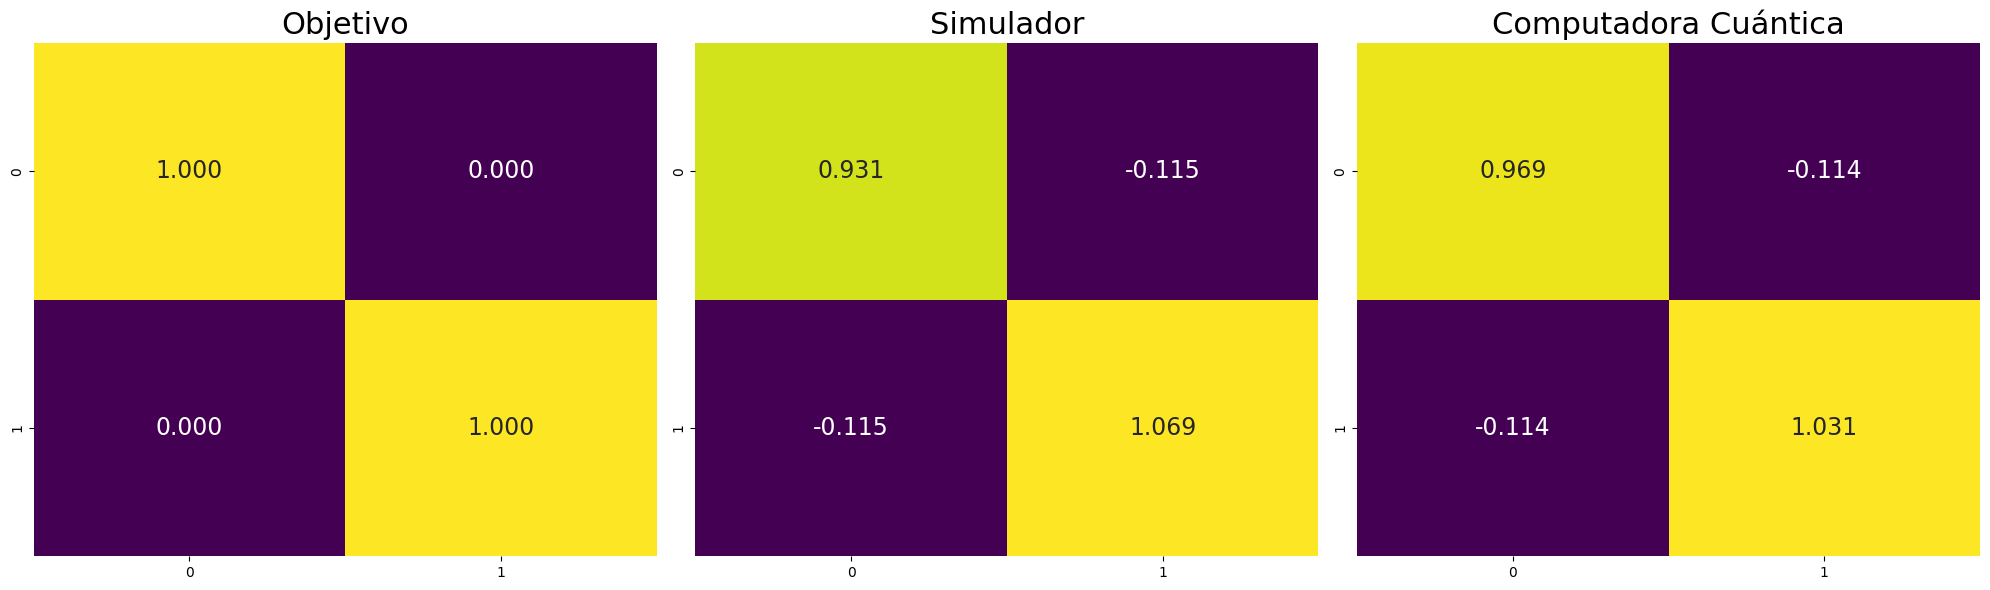
\includegraphics[width=\linewidth,height=0.45\textheight,keepaspectratio]{imagenes/ident_comp_0.1.png}
    \caption{$p=0.1$}
    \label{fig:2x2_01}
  \end{subfigure}\hfill
  \begin{subfigure}[t]{0.50\textwidth}
    \centering
    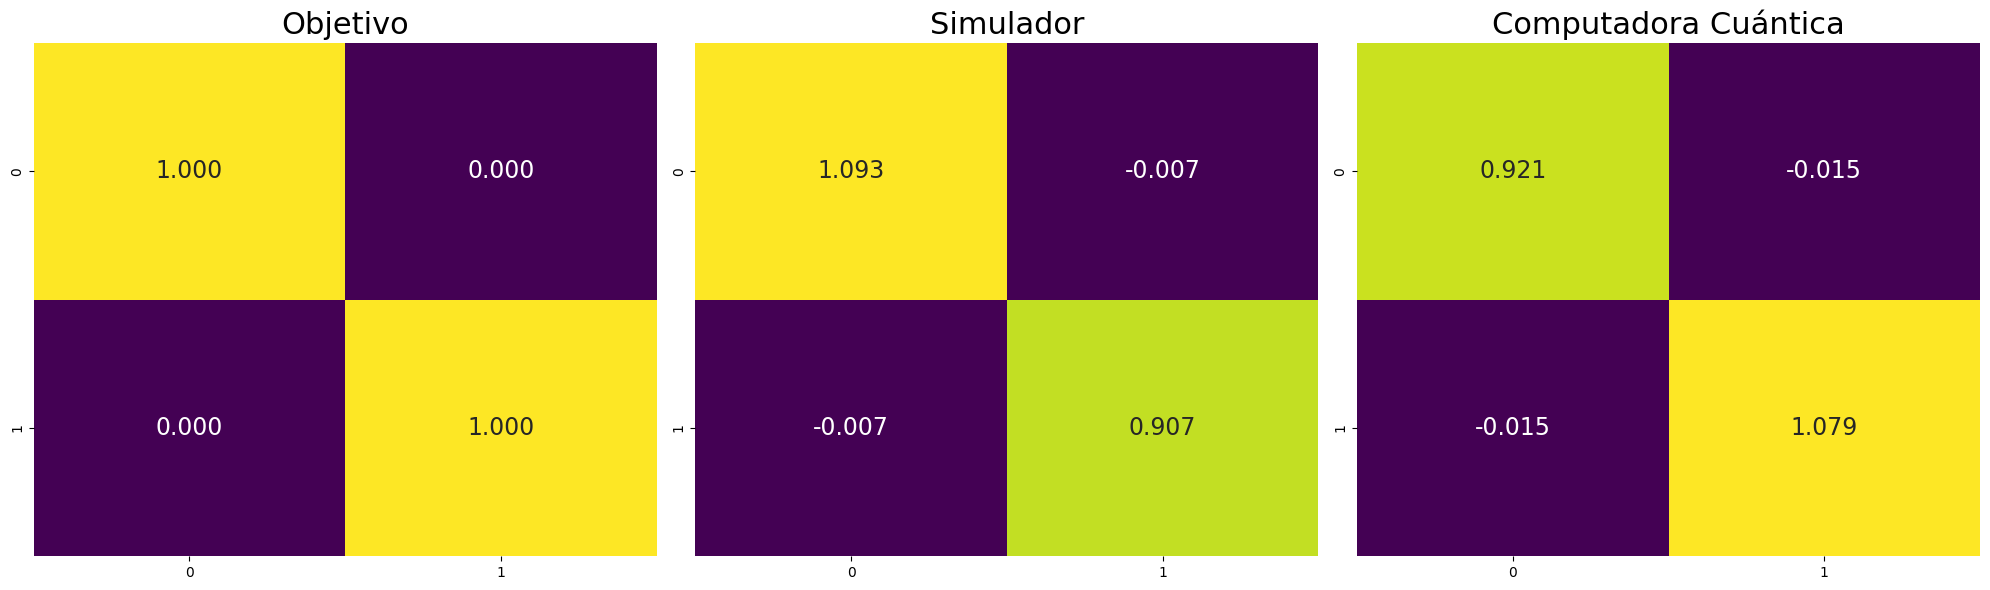
\includegraphics[width=\linewidth,height=0.45\textheight,keepaspectratio]{imagenes/ident_comp_0.5.png}
    \caption{$p=0.5$}
    \label{fig:2x2_02}
  \end{subfigure}

  \par\vspace{0.6em}

  % ===== Fila 2 =====
  \begin{subfigure}[t]{0.50\textwidth}
    \centering
    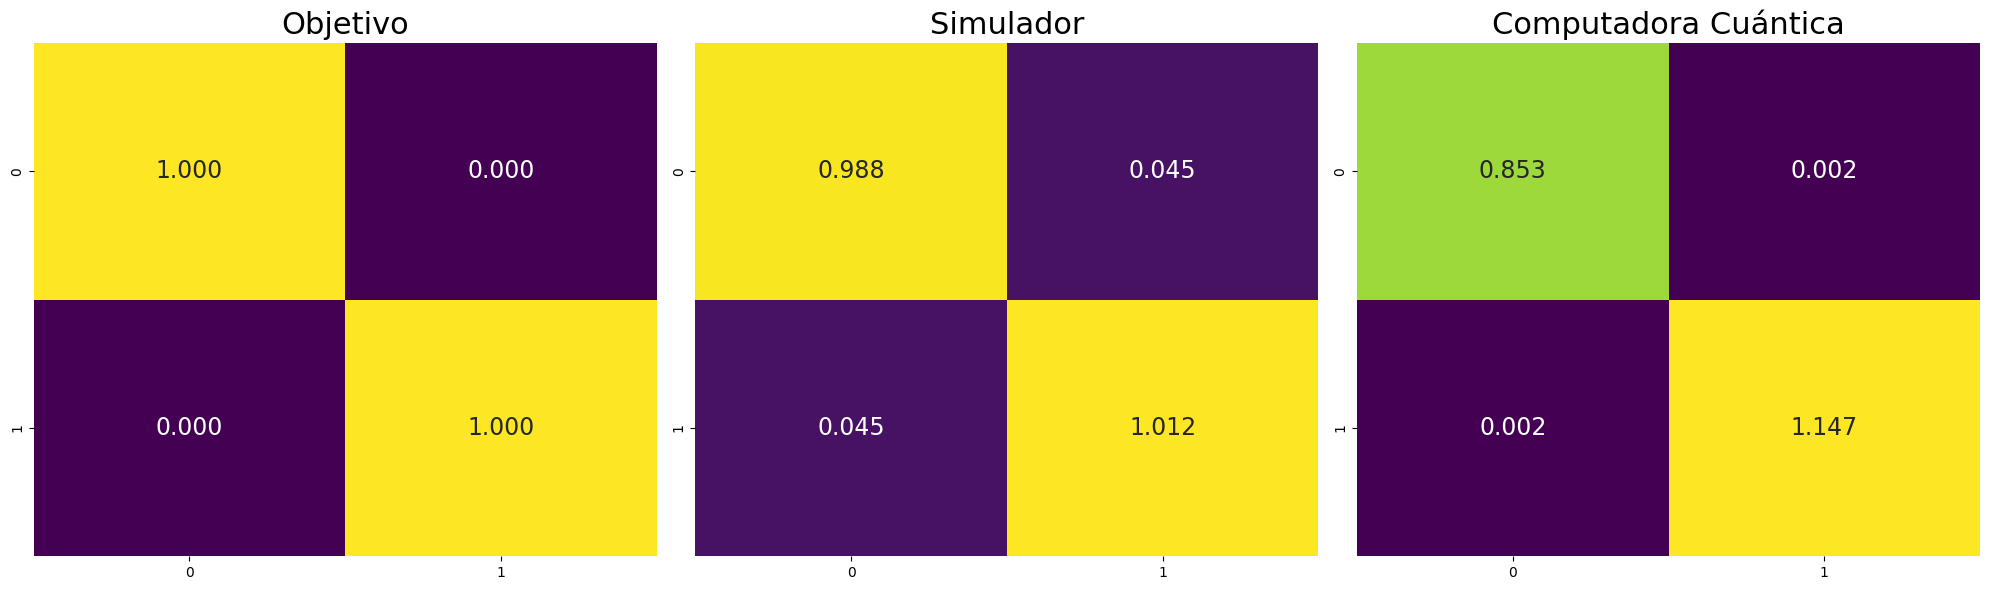
\includegraphics[width=\linewidth,height=0.45\textheight,keepaspectratio]{imagenes/ident_comp_0.7.png}
    \caption{$p=0.7$}
    \label{fig:2x2_03}
  \end{subfigure}\hfill
  \begin{subfigure}[t]{0.50\textwidth}
    \centering
    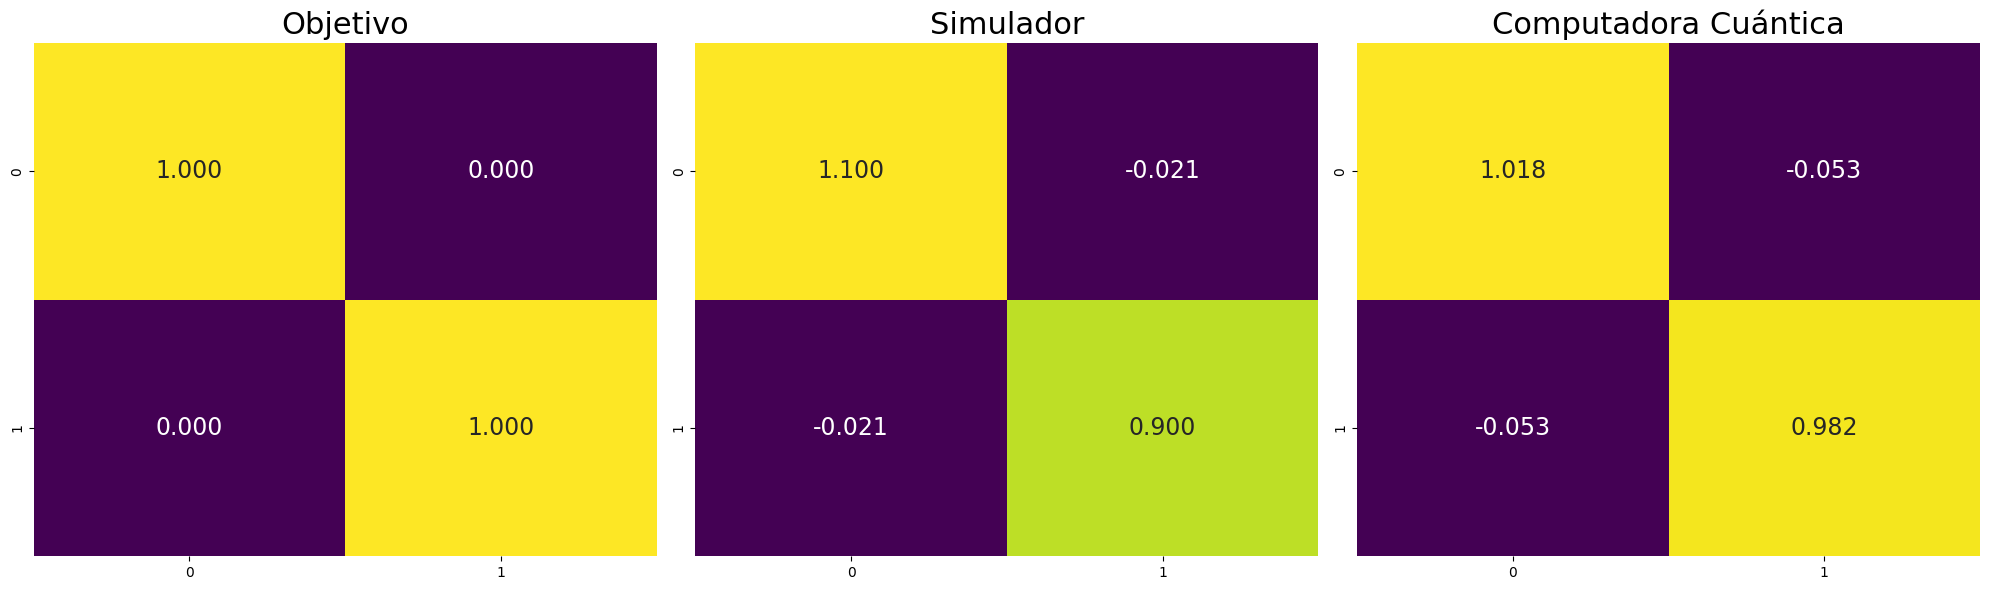
\includegraphics[width=\linewidth,height=0.45\textheight,keepaspectratio]{imagenes/ident_comp_0.9.png}
    \caption{$p=0.9$}
    \label{fig:2x2_04}
  \end{subfigure}

  % \caption{Comparación 2×2 (texto opcional para título general).}
  \label{fig:2x2_grid}
\end{figure}
\end{frame}

\begin{frame}{Resultados}
\framesubtitle{Tendencias}
    \begin{columns}[c] % The "c" option specifies centered vertical alignment while the "t" option is used for top vertical alignment

        \column{.50\textwidth} % Left column and width
        \begin{figure}[h]
                \centering
                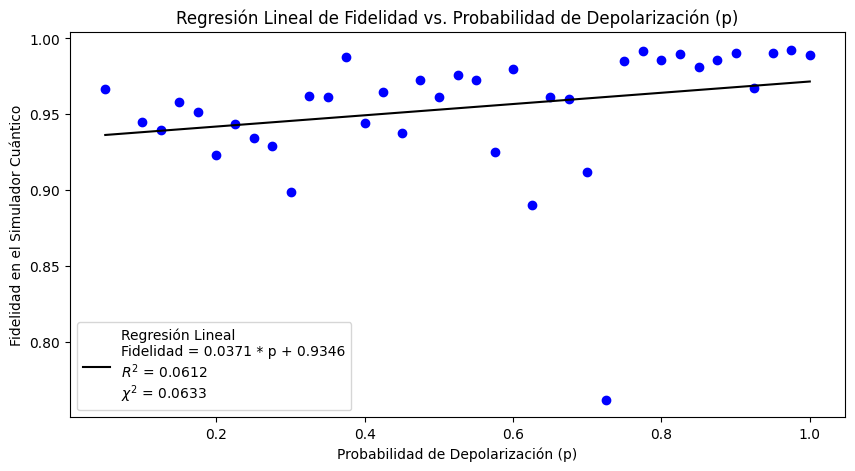
\includegraphics[scale=0.34]{imagenes/Regresion Fidelidad sim.png}
            \end{figure}
        \begin{itemize}
            \item $F_{proc\_sim}(p) = 0.0371 \cdot p + 0.9346$
            \item $R^2 = 0.0612$
            \item $\chi^2 = 0.0633$
        \end{itemize}
        \column{.50\textwidth} % Right column and width
            \begin{figure}[h]
                \centering
                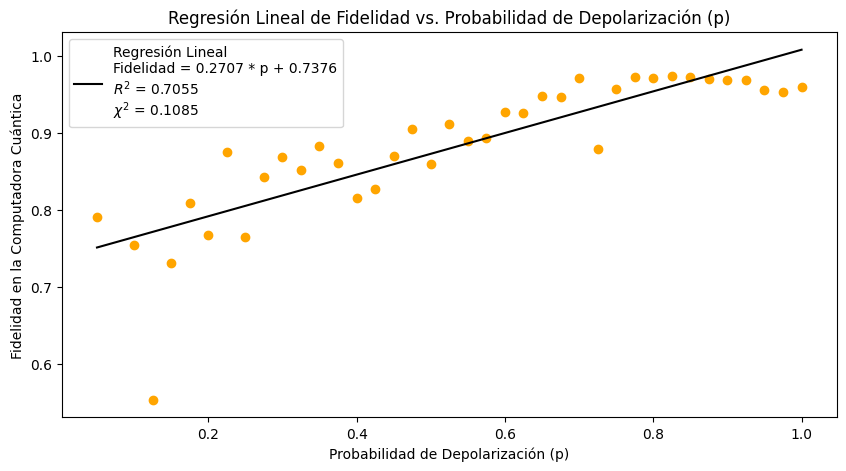
\includegraphics[scale=0.34]{imagenes/Regresion Fidelidad_qc.png}
            \end{figure}
            \begin{itemize}
            \item $ F_{proc\_qc}(p) = 0.2707 \cdot p + 0.7376$
            \item $R^2 = 0.7055$
            \item $\chi^2 = 0.1085$
        \end{itemize}
    \end{columns}
\end{frame}

\begin{frame}{Resultados}
 \framesubtitle{Desviación estándar}
\begin{figure}[h!] % {{{
    \centering
    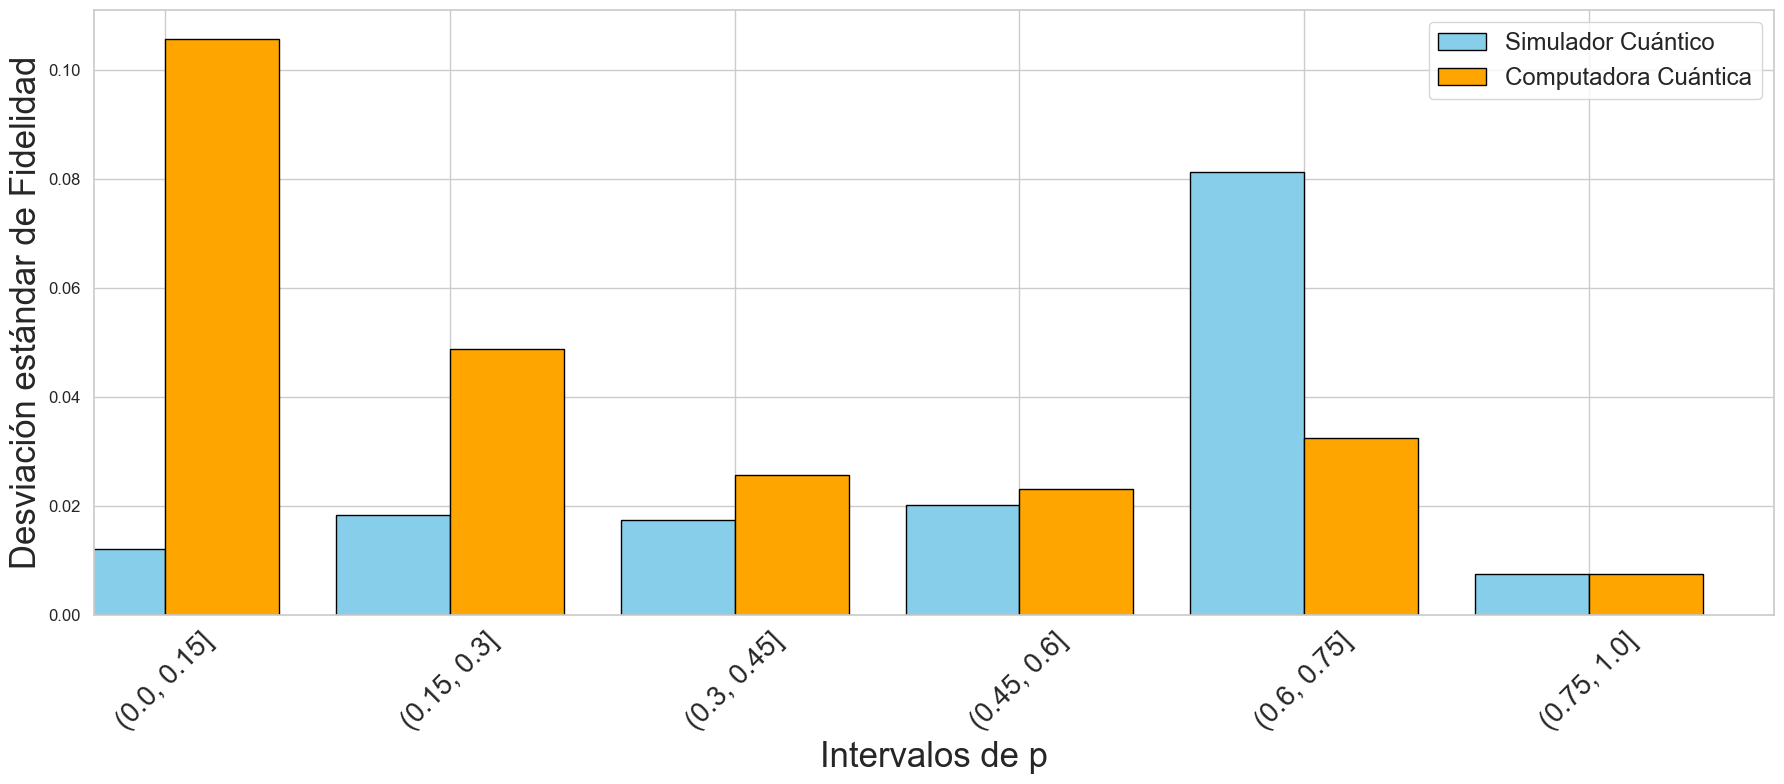
\includegraphics[width=0.95\linewidth]{imagenes/Comparacion_desviaciones.png}
    % \caption[Comparación de desviación estándar para resultados de fidelidad de proceso]{Comparación de desviación estándar entre los resultados de la fidelidad de proceso entre la matriz de Choi esperada, la computadora cuántica \texttt{ibm\_kyoto} (color naranja) y el simualdor cuántico (color azul) \texttt{AerSimualtor()}. La desviación estándar se calcula sobre los valores de fidelidad en el intervalo de $p$. \textbf{Fuente:} elaboración propia.}
    \label{fig:comparacion_desviaciones}
\end{figure} % }}}
\end{frame}

\begin{frame}{Resultados}
\framesubtitle{Matrices de Choi}
\begin{figure}
  \centering
  \begin{subfigure}[t]{0.65\textwidth}
    \centering
    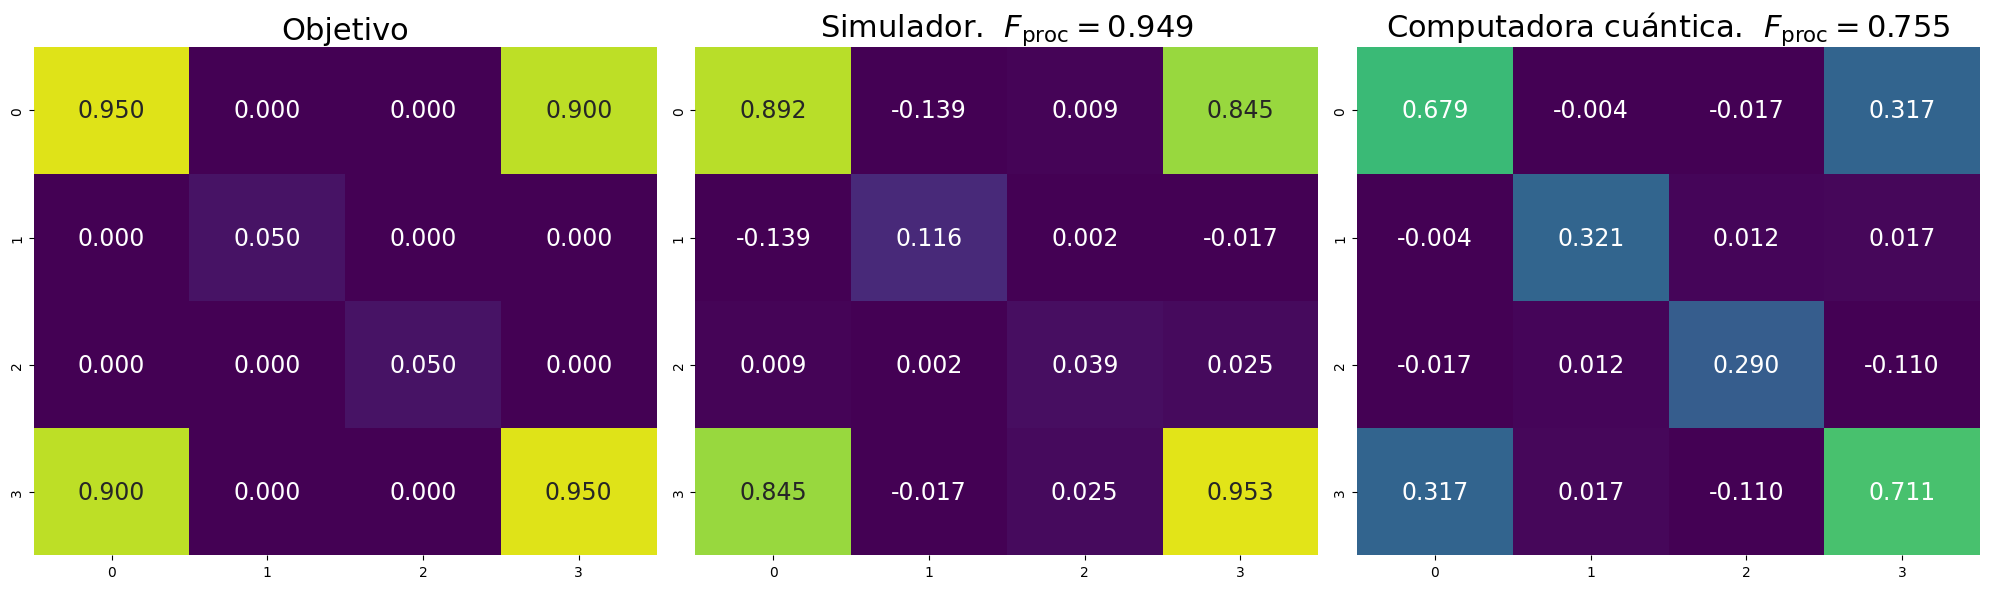
\includegraphics[width=\linewidth,height=0.60\textheight,keepaspectratio]{imagenes/comp_choi_p0.1.png}
    \caption{Resultados para $p=0.1$}
    \label{fig:1x2_A}
  \end{subfigure}\hfill
  \begin{subfigure}[t]{0.65\textwidth}
    \centering
    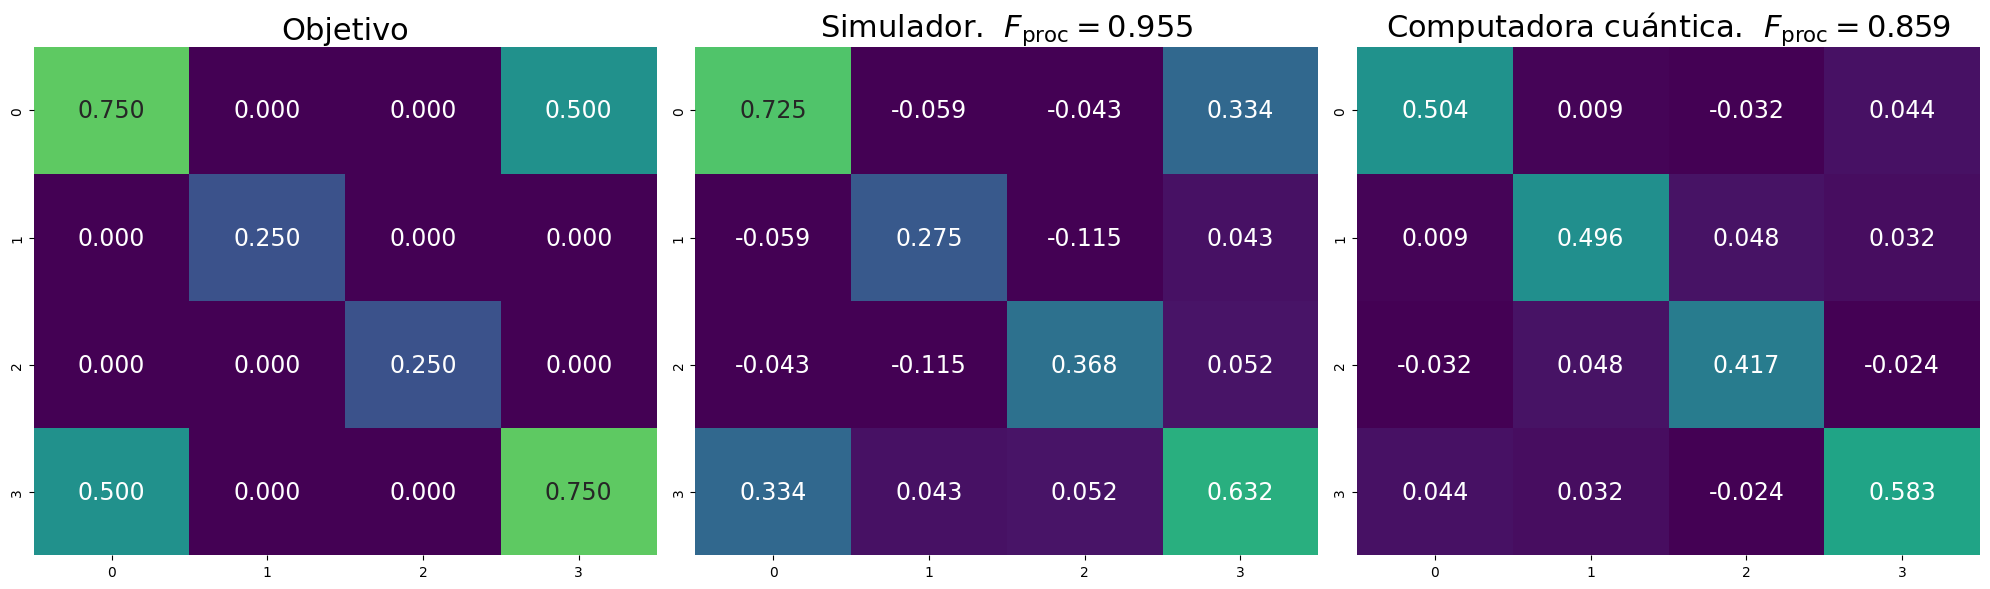
\includegraphics[width=\linewidth,height=0.60\textheight,keepaspectratio]{imagenes/comp_choi_p0.5.png}
    \caption{Resultados para $p=0.5$}
    \label{fig:1x2_B}
  \end{subfigure}
  % \caption{}
\end{figure}
\end{frame}

\begin{frame}{Resultados}
\framesubtitle{Matrices de Choi}

\begin{figure}
  \centering
  \begin{subfigure}[t]{0.65\textwidth}
    \centering
    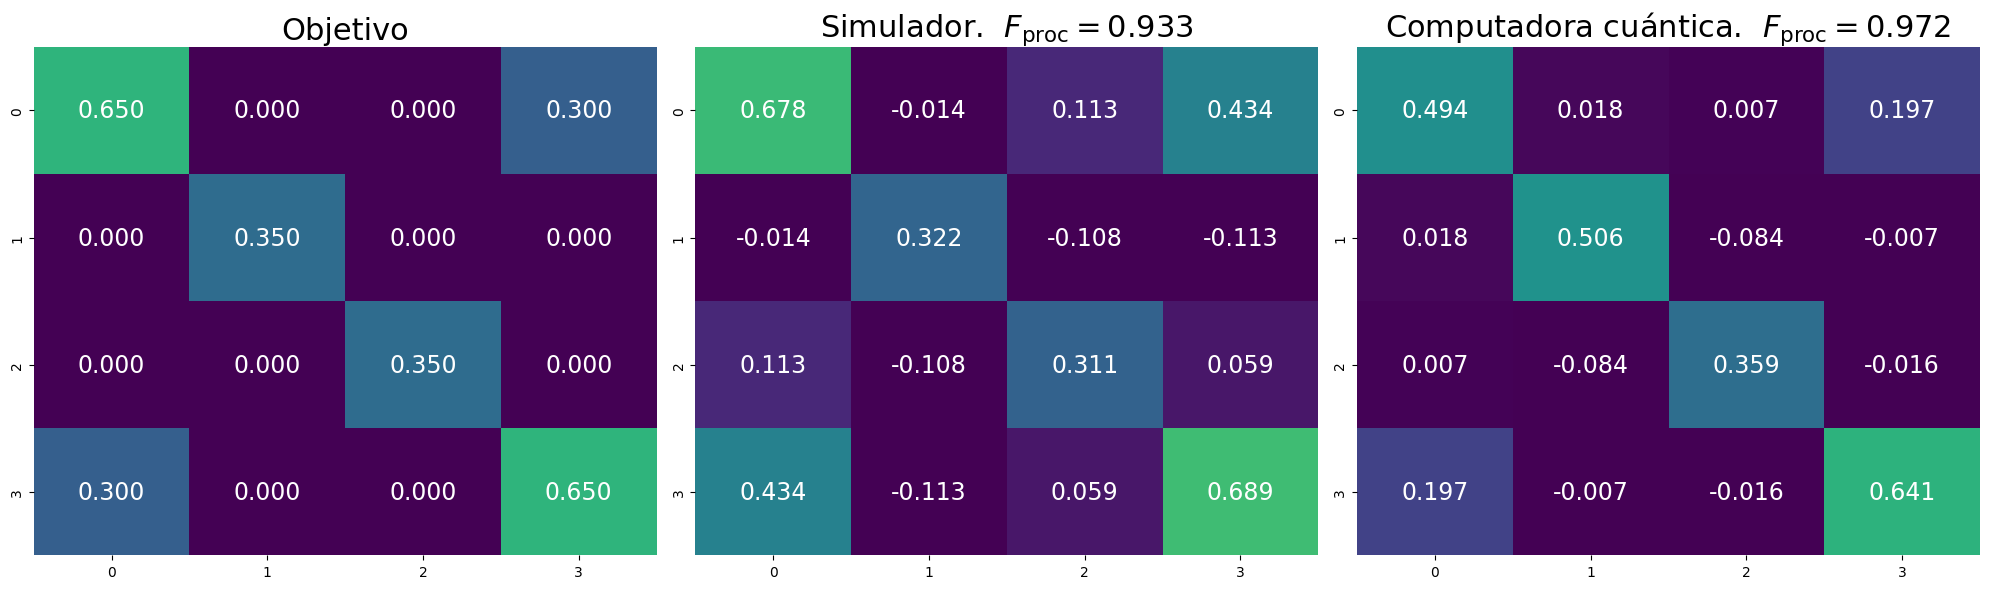
\includegraphics[width=\linewidth,height=0.50\textheight,keepaspectratio]{imagenes/comp_choi_p0.7.png}
    \caption{Resultados para $p=0.7$}
    \label{fig:1x2_A}
  \end{subfigure}\hfill
  \begin{subfigure}[t]{0.65\textwidth}
    \centering
    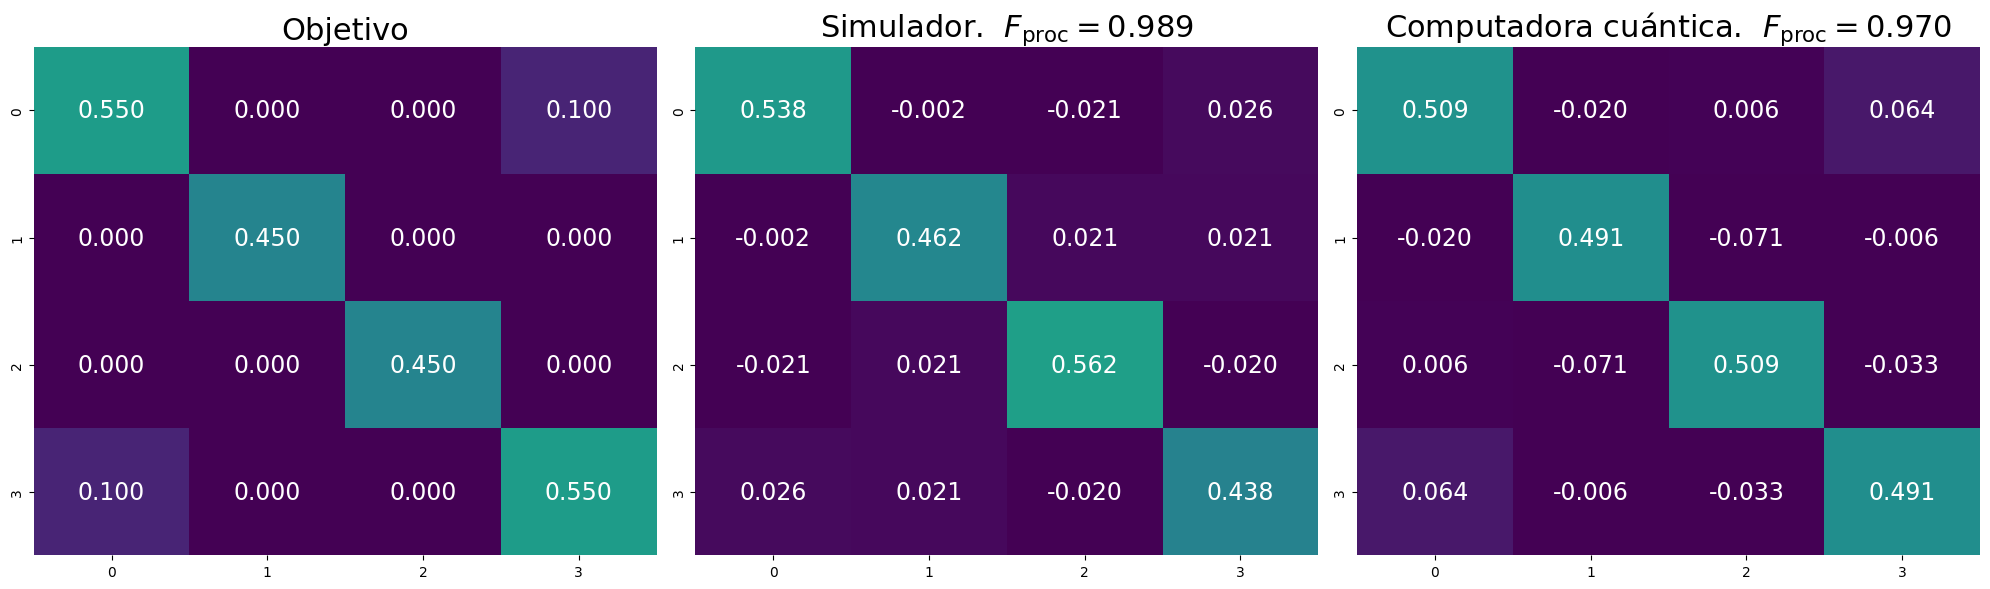
\includegraphics[width=\linewidth,height=0.50\textheight,keepaspectratio]{imagenes/comp_choi_p0.9.png}
    \caption{Resultados para $p=0.9$}
    \label{fig:1x2_B}
  \end{subfigure}
  % \caption{}
\end{figure}
\end{frame}




%     \begin{table}
%         \begin{tabular}{l l l}
%             \toprule
%             \textbf{Treatments} & \textbf{Response 1} & \textbf{Response 2} \\
%             \midrule
%             Treatment 1         & 0.0003262           & 0.562               \\
%             Treatment 2         & 0.0015681           & 0.910               \\
%             Treatment 3         & 0.0009271           & 0.296               \\
%             \bottomrule
%         \end{tabular}
%         \caption{Table caption}
%     \end{table}
% \end{frame}

\section{Conclusiones y trabajo a futuro}
%------------------------------------------------



\begin{frame}{Conclusiones}
\begin{itemize}
    \item Se implementó el canal despolarizante de un qubit usando algoritmos variacionales cuánticos (VQA), mediante un \textit{hardware-efficient ansatz} optimizado por fidelidad de proceso.
    
    \item Las ejecuciones en simulador cuántico mostraron fidelidades superiores a 0.900 con baja variabilidad, confirmando la efectividad del enfoque en entornos ideales.
    
    \item En la computadora cuántica (\texttt{ibm\_kyoto}), se observó una tendencia creciente en la fidelidad conforme aumentó la probabilidad de despolarización $p$, con una regresión lineal de pendiente $m = 0.2707$ y $R^2 = 0.7055$.
    
    \item La reducción de variabilidad con $p$ sugiere mayor tolerancia al ruido en estados más mixtos; sin embargo, las matrices de Choi indicaron que el hardware preserva coherencias no triviales en bajas despolarizaciones.
    
    % \item El estudio demuestra que los VQA son una herramienta prometedora para simular canales cuánticos en hardware cuántico, aunque su desempeño está condicionado por el ruido y la calidad del dispositivo.
\end{itemize}
\end{frame}

%------------------------------------------------

% \begin{frame}{References}
%     \footnotesize
%     \bibliography{reference.bib}
%     \bibliographystyle{apalike}
% \end{frame}

%------------------------------------------------


\end{document}

% \begin{frame}{Table}
%     \begin{table}
%         \begin{tabular}{l l l}
%             \toprule
%             \textbf{Treatments} & \textbf{Response 1} & \textbf{Response 2} \\
%             \midrule
%             Treatment 1         & 0.0003262           & 0.562               \\
%             Treatment 2         & 0.0015681           & 0.910               \\
%             Treatment 3         & 0.0009271           & 0.296               \\
%             \bottomrule
%         \end{tabular}
%         \caption{Table caption}
%     \end{table}
% \end{frame}

%----------------------------------------------------------------------------------------





